\documentclass[tikz,border=5pt]{standalone}
\usepackage[utf8]{inputenc}
\usepackage[T1]{fontenc}
\usepackage{lmodern,amsmath,amssymb}
\usepackage[american]{circuitikz}
\usepackage{pgfplots}
\pgfplotsset{compat=1.18}
\usetikzlibrary{circuits.logic.US,positioning,calc,arrows.meta,patterns,shapes.geometric}
\definecolor{Primary}{HTML}{1F77B4}
\begin{document}
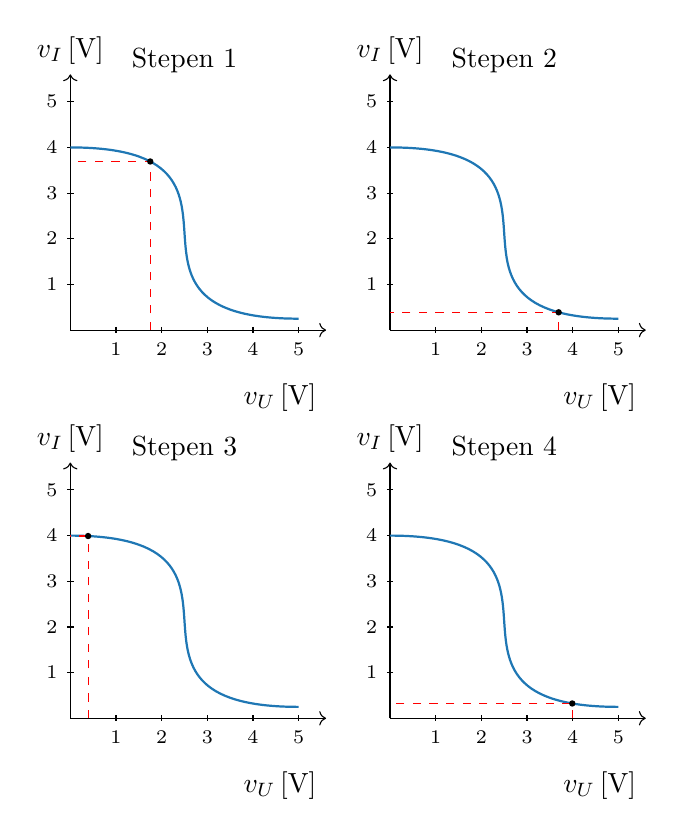
\begin{tikzpicture}[scale=.58]\begin{scope}[xshift=0cm,yshift=0cm]\draw[->] (0,0)--(5.6,0);\node[anchor=north east]at(5.6,-.95){$v_U\,[\mathrm V]$};\draw[->] (0,0)--(0,5.6) node[above]{$v_I\,[\mathrm V]$};\foreach \x in {1,...,5}{\draw (\x,.07)--(\x,-.07) node[below,font=\scriptsize]{\x};\draw (.07,\x)--(-.07,\x) node[left,font=\scriptsize]{\x};}\draw[Primary,thick] (0,4).. controls (4.75,4) and (.25,.25)..(5,.25);\draw[dashed,red] (1.75000,0)|-(0,3.69203);\fill (1.75000,3.69203) circle(2pt);\node at (2.5,5.9) {Stepen 1};\end{scope}\begin{scope}[xshift=7cm,yshift=0cm]\draw[->] (0,0)--(5.6,0);\node[anchor=north east]at(5.6,-.95){$v_U\,[\mathrm V]$};\draw[->] (0,0)--(0,5.6) node[above]{$v_I\,[\mathrm V]$};\foreach \x in {1,...,5}{\draw (\x,.07)--(\x,-.07) node[below,font=\scriptsize]{\x};\draw (.07,\x)--(-.07,\x) node[left,font=\scriptsize]{\x};}\draw[Primary,thick] (0,4).. controls (4.75,4) and (.25,.25)..(5,.25);\draw[dashed,red] (3.69203,0)|-(0,0.38954);\fill (3.69203,0.38954) circle(2pt);\node at (2.5,5.9) {Stepen 2};\end{scope}\begin{scope}[xshift=0cm,yshift=-8.5cm]\draw[->] (0,0)--(5.6,0);\node[anchor=north east]at(5.6,-.95){$v_U\,[\mathrm V]$};\draw[->] (0,0)--(0,5.6) node[above]{$v_I\,[\mathrm V]$};\foreach \x in {1,...,5}{\draw (\x,.07)--(\x,-.07) node[below,font=\scriptsize]{\x};\draw (.07,\x)--(-.07,\x) node[left,font=\scriptsize]{\x};}\draw[Primary,thick] (0,4).. controls (4.75,4) and (.25,.25)..(5,.25);\draw[dashed,red] (0.38954,0)|-(0,3.99076);\fill (0.38954,3.99076) circle(2pt);\node at (2.5,5.9) {Stepen 3};\end{scope}\begin{scope}[xshift=7cm,yshift=-8.5cm]\draw[->] (0,0)--(5.6,0);\node[anchor=north east]at(5.6,-.95){$v_U\,[\mathrm V]$};\draw[->] (0,0)--(0,5.6) node[above]{$v_I\,[\mathrm V]$};\foreach \x in {1,...,5}{\draw (\x,.07)--(\x,-.07) node[below,font=\scriptsize]{\x};\draw (.07,\x)--(-.07,\x) node[left,font=\scriptsize]{\x};}\draw[Primary,thick] (0,4).. controls (4.75,4) and (.25,.25)..(5,.25);\draw[dashed,red] (3.99076,0)|-(0,0.32443);\fill (3.99076,0.32443) circle(2pt);\node at (2.5,5.9) {Stepen 4};\end{scope}\end{tikzpicture}
\end{document}
